\section{Related Work}

The use of scientific visualization in immersive environments is simply natural, while tactically important for scientific discovery, product design and data analysis.
There are several high quality scientific visualization virtual reality applications created from scratch using OpenGL directly~\cite{Billen:2008, LaViola:2007, Schulze:2001, Rantzau:1998} including the stunning GPU accelerated hybrid volume and glyph approach for molecular dynamics visualization in the CAVE2 by Reda et al~\cite{Reda:2013}.
These are certainly exemplary and valuable applications.
However, when building immersive applications, much like desktop applications, with scientific requirements, it is often more efficient to leverage the open source visualization toolkit (VTK)~\cite{Schroeder:2004}.

Throughout the past two decades, several research teams and developers have integrated VTK with immersive environments to varying degrees of success.
Four fundamental approaches are available to bring VTK into an
immersive rendering system:

\begin{compactitem}
\item Geometry transport;
\item OpenGL context sharing;
\item VR toolkit embedding; and
\item OpenGL intercept.

\end{compactitem}

Our recent enhancements to the VTK platform contain solutions for the desired integration that present a number of contributions, and, therefore, we review related work for these areas.

\textbf{\textit{Geometry transport}}
An early approach to VTK-VR integration was the \texttt{vtkActorToPF} library~\cite{Leigh98limbo/vtk}.
In this method, the generation of visualization geometry is decoupled from
the rendering of the geometry (see Figure~\ref{fig:vtkActorToPF}). 
VTK generates the geometry in the form of actors that consist of polygons and properties.
\texttt{vtkActorToPF} transforms these actors into pf-Geodes (nodes) that are included in a Performer (OpenSceneGraph) scene graph. The geometry is created by VTK, and the scene graph is rendered without VTK. Only geometry is transformed. Cameras, lights, rendering and interaction are not incorporated. Several applications utilized the equivalent \texttt{vtkActorToOSG} for an OpenSceneGraph-based scene graph~\cite{VE-Suite:2016} or directly into OpenGL~\cite{Ohno:2006}. Others have used VTK in a preprocessing step to produce geometries or textures eliminating the need for a direct connection to VTK\cite{Bivins:2005}.

\begin{figure}[h!]
  \centering
  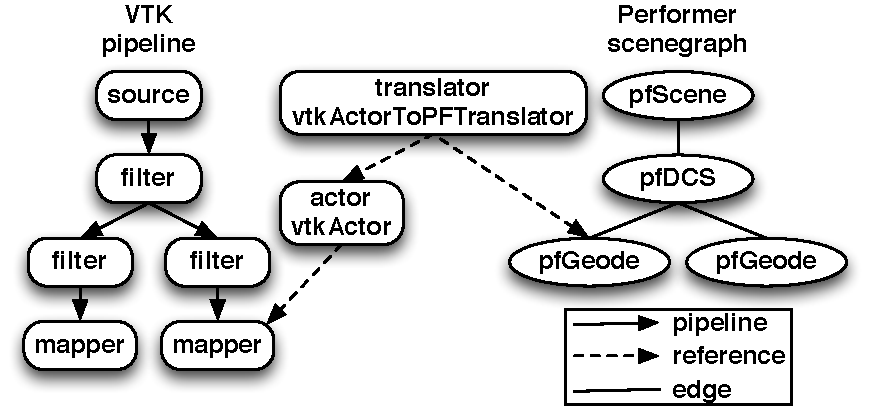
\includegraphics[width=\linewidth]{images/vtkActorToPF.pdf}
  \caption{VTK, vtkActorToPF and Performer interaction diagram. (Recreated from Paul Rajlich~\ref{fig:vtkActorToPF}.)}
  \label{fig:vtkActorToPF}
\end{figure}

VTK can be used to create, transport and save geometry without rendering. As effective as this approach can be, the loose coupling of VTK and a VR toolkit creates more obstacles than benefits from an application developers perspective, and is not built upon by this work.

\textbf{\textit{OpenGL context sharing}} Rather than share just the VTK geometry, the application developer would like to use all of the VTK API from within their immersive application.
In VTK, the renderer and render window classes are responsible for rendering scenes.
VTK creates it's own window and associates an OpenGL context with that window to be used by the renderer.
An OpenGL context represents: all of the state; the default framebuffer; and everything affiliated with OpenGL with respect to the renderer, window and application.
The application developer would simply like to share the OpenGL context from the VR Toolkit with a third party rendering software (e.g. Delta3D~\cite{McDowell:2006}, OpenSceneGraph~\cite{Wang:2010} and VTK). 

In previous work, by Sherman et al.~\cite{Sherman:2010} and others, Delta3D
and OpenSceneGraph were quickly modified to instead use windows and associated
OpenGL contexts of a VR integration library such as Vrui~\cite{Kreylos:2006}.
% in final paper can mention FreeVR.
These solutions are generally limited in their integration.
Specifically, a rendering library that is unaware of the actual
viewing matrix will generally not calculate lighting correctly, and
picking input operations do not conform to the shifted rendering.

Our \texttt{vtkRenderingExternal} VTK module formalizes this integration providing lights, interaction and picking connectivity lacking in other implementations, while allowing the application developer complete access to the VTK pipeline.

\textbf{\textit{VR Toolkit embedding}} A similarly time-proven approach is based on the modification of the VTK renderer and render window~\cite{van2000vista, Hannema:2001, Shamonin02vtkcave, Belleman:2003}.
To render in an immersive environment, derived classes of the
\texttt{vtkRenderer} and \texttt{vtkRenderWindow} are created, which depends on fundamental calls to the VR toolkit.
Thus, VTK-based applications can simply exchange these two items to run on the desktop or immersive environment.
VTK has evolved significantly over the years, as have the diversity of virtual reality products.
vtkCave~\cite{Tufo:1999}, for the CAVELib~\cite{CAVELib:2016}, followed by
vjVTK~\cite{Blom:2006} and VR JuggLua~\cite{Pavlik:2012}, for
VRJuggler~\cite{Bierbaum:2001}, created third party software essentially
deriving \texttt{vtkRenderWindow} and \texttt{vtkRenderer} classes, but, from
outside of VTK; lighting and interaction were not shared and resulted in troublesome behavior.

In this work, we've created a new VTK module based on OpenVR~\cite{OpenVR:2016}.
OpenVR is an application programming interface (API) developed by Valve for supporting their SteamVR ecosystem, compatible with the HTC Vive and other virtual reality hardware~\cite{Road2VR:2015}.
The OpenVR module supports several immersive environments now without the issues faced by previous work, and provides a template for embedding other VR Toolkits within VTK in the future.

\textit{\textbf{OpenGL intercept}}
A fourth possible means for melding VTK into a virtual environment system
is the \textit{OpenGL intercept} method
~\cite{Humphreys:2001,Humphreys:2002,Zielinski:2014,TechViz:2016,Conduit:2016}.
Here, at runtime, middleware is inserted between the application and the graphics card.
With this technique, closed-source applications can be rendered with
the head-tracked perspective rendering overriding the internal view matrix
to provide the virtual reality experience.
Thus, this technique enables basic desktop tools to be used with an
immersive interface | albeit a limited interface given the open-loop nature of
grabbing the rendering, but not connecting back to the parameter interface.
Yet, the perspective rendering alone can be extremely valuable and allow
scientists, engineers or medical researchers to interact with their desktop
tools in a whole new way. However, many of these methods lack full functionality in the immersive environments, which limits the usefulness to end users.
Pure OpenGL, without any modifications or additions,  is sure to work using interception.
The difficulty of using intercept methods is that they require more coding
and tagging, and are not guaranteed to work at all, and this is becoming
more difficult with OpenGL 3.0+, especially when using a core OpenGL profile.

%In contrast to the OpenGL intercept method, the work in this paper is for the application developer, and there is no intention to eliminate the need to write code.
%%Rather ...?

\textit{\textbf{Enhanced performance}} Near real-time update of scientific visualization metaphors is crucial in immersive environments.
The field has seen several proposed solutions from decoupling rendering, and processing to parallel visualization~\cite{Bryson:1996, van2000vista}.
This effort stands apart from all these previous efforts, which valiant
as they were, ultimately have been lost to time as VTK has continued to
evolve, making it difficult for tacked-together components to remain in
sync with the API.
Rather, by providing rendering access from within the VTK API itself, new
tools can rely on a stability that hasn't been available for techniques
that perform functions outside the bounds of the API design, often accessing
internal features that do not have the assurance of stability.
As a commercially supported open-source tool, VTK's rendering performance is
continually being advanced.
VTK has been around since 1993 with over one hundred thousand repository commits from over two-hundred and fifty contributors.
Having the latest algorithm implementation requires using the existing implementation in VTK or contributing the algorithm to VTK.

We present recent enhancements to VTK that significantly impact immersive
environment application development. The OpenGL 3.2+ pipeline, described in Hanwell et al~\cite{Hanwell:2015}, provides the most dramatic improvement in performance. We have supplemented this work with Bavoil and Myers dual depth peeling~\cite{Bavoil:2008} and symmetric multiprocessing (SMP) tools and algorithms to address the performance issues for transparent geometry and computationally intense algorithms (e.g. isosurfaces).

Finally, our work will eventually allow application developers to leverage portable threaded data parallel algorithms capable of running on next generation hardware from VTK-m~\cite{Moreland:2016}. VTK-m has shown impressive results in its first two years of development, and, as the number of filters available in VTK-m's repository grows, the plan is to make them available in the next major release of VTK. Thus, if VTK-m is contained in VTK, then applications developed using the integrations described in this paper can use it.


